%%%%%%%%%%%%%%%%%%%%%%%%%%%%%%%%%%%%%%%%%%%%%%%%%%%%%%%%%%%%%%%%%%%%%%%%%%%%%%%%
%                                                                              %
%            A Painless Introduction to Programming UAMMD Modules              %
%                           Chapter 3: Measuring                               %
%                                                                              %
%                          Marc Meléndez Schofield                             %
%                                                                              %
%%%%%%%%%%%%%%%%%%%%%%%%%%%%%%%%%%%%%%%%%%%%%%%%%%%%%%%%%%%%%%%%%%%%%%%%%%%%%%%%

The first two chapters have given you more than enough material to create your 
own simulations and use the output to make videos of spheres flying around and 
colliding in your own virtual world. But scientists aim at describing the real 
world, and that involves measuring interesting quantities in your system and 
relating them to material objects.

\section{Energy and linear momentum}

Physical simulations commonly measure energy. Unexpected fluctuations or drifts 
in the energy often warn us of something askew in our code. Take our bouncing 
rubber ball from the introduction. Its mechanical energy,
\begin{equation*}
  E = \frac{1}{2} m \|\mathbf{v}\|^2 + m|g|y,
\end{equation*}
should remain constant while it flies freely. The absolute value $|g|$ appears 
here instead of plain $g$ because, if you remember, we defined the acceleration 
of gravity as $g = -9.8\ \mathrm{m/s}^2$ in our code. On impact, the ball 
reduced its speed slightly, so we expect a sudden drop in $E$ every time 
the ball hits the floor. As it bounces time and again, leaking more and more 
energy, $E$ will tend towards zero.

Due to numerical rounding in the operations, we shouldn't expect a perfect 
conservation of energy but we obviously want to keep energy fluctuations low, 
below one percent, say. If you have managed to code the algorithm correctly, you 
can usually decrease energy fluctuations further by choosing smaller time steps.

Let's verify our predictions about the bouncing ball program by changing the 
output section. We'll set the mass to $100$ grams.
\begin{lstlisting}
%! codeblock: rubberBallEOutput
    if(printEverynSteps > 0
       && step % printEverynSteps == 0) {

      float m = 0.1; /* Mass */

      /* Mechanical energy */
      float E = 0.5*m*(v[0]*v[0] + v[1]*v[1]) - m*g*r[1];

      cout<<step*dt<<" "<<r[0]<<" "<<r[1]<<" "<<E<<endl;
    } //!
%! codeblockend !//
\end{lstlisting}
Note that I wrote \texttt{-m*g*r[1]} instead of \texttt{+m*g*r[1]} due to the 
negative value of \texttt{g}. Figure \ref{rubberBallE} plots the result, which 
agrees with our predictions precisely.

\begin{figure}
  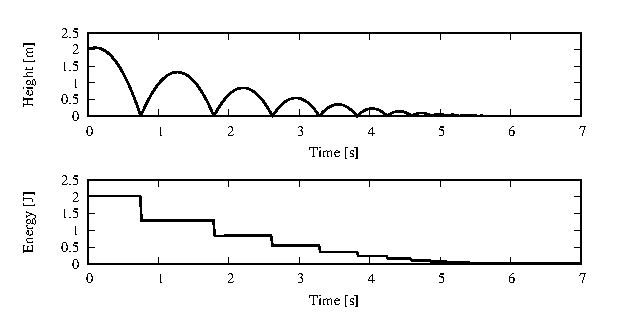
\includegraphics[width = \textwidth]{figures/rubberBallE.eps}
  \caption{\label{rubberBallE}Height (\textit{top}) and mechanical energy 
           (\textit{bottom}) of a one-hundred-gram bouncing ball versus time. 
           The energy remains constant with the ball in free flight, but a 
           fraction is lost when the ball hits the ground.}
\end{figure}

\begin{comment}
rubberBallE.cpp differs only from rubberBall.cpp in the code snippet mentioned 
above.
%! codefile: code/rubberBallE.cpp
# include <iostream>

using std::cout;
using std::endl;

int main(int argc, char * argv[])
{
  /* State of the rubber ball */
  float r[2]; /* Position (measured in metres) */
  float v[2]; /* Velocity (in metres/second) */

  float g = -9.8; /* Acceleration of gravity (in m/s^2) */

  /* Integration parameters */
  int nsteps = 10000; /* Number of time steps to calculate */
  float dt = 0.001; /* Size of time step (in seconds) */
  int printEverynSteps = 20;

  /* Initial conditions */
  r[0] = 0;
  r[1] = 2;
  v[0] = 0.5;
  v[1] = 1;

  /* Euler integration of the equations of motion */
  for(int step = 0; step <= nsteps; ++step) {
    /* New position */
    r[0] = r[0] + v[0]*dt;
    r[1] = r[1] + v[1]*dt;

    /* New velocity */
    v[1] = v[1] + g*dt;

    /* Deal with collisions */
    if(r[1] <= 0 && v[1] < 0) {
      v[0] = 0.9*v[0];
      v[1] = -0.8*v[1];
    }

    /* Output state */
    %! codeinsert: rubberBallEOutput
  }
  cout<<"# Simulated time: "<<nsteps*dt<<" seconds. #"<<endl;
  return 0;
}
%! codeend
\end{comment}

Returning to UAMMD, let's write a function that outputs the total energy of the 
system. Each interactor has a \texttt{sumEnergy} method that calculates the 
potential energy due to corresponding interaction for each particle and adds it 
to the energy vector that we access with \texttt{getEnergy}. You can add the 
kinetic energy by calling the interactor's \texttt{sumEnergy}.

To begin with, our new \texttt{getTotalEnergy} function will clear the energy 
vector and initialize the \texttt{totalEnergy} variable to zero.
\begin{lstlisting}
%! codeblock: getTotalEnergy
double getTotalEnergy(std::shared_ptr<Integrator> integrator,
                      std::shared_ptr<ParticleData> particles){
  {
    auto energy
      = particles->getEnergy(access::location::cpu,
                             access::mode::write);
    std::fill(energy.begin(), energy.end(), real(0.0));
  }

  double totalEnergy = 0; //!
  %! codeinsert: getKineticEnergy
  %! codeinsert: getPotentialEnergy
  %! codeinsert: reduceEnergyVector
%! codeblockend !//
\end{lstlisting}
Next, it stores the kinetic energies in the particle energy vector.
\begin{lstlisting}
%! codeblock: getKineticEnergy
  integrator->sumEnergy(); //!
%! codeblockend !//
\end{lstlisting}
After that, it adds in the potential energies from interactions.
\begin{lstlisting}
%! codeblock: getPotentialEnergy
  for(auto interactor: integrator->getInteractors()){
    interactor->sumEnergy();
  } //!
%! codeblockend !//
\end{lstlisting}
Finally, we accumulate all the values in the energy vector and return the grand 
total.
\begin{lstlisting}
%! codeblock: reduceEnergyVector
  {
    auto energy
      = particles->getEnergy(access::location::cpu,
                             access::mode::read);
    for(int i = 0; i < particles->getNumParticles(); ++i) {
      totalEnergy += energy[i];
    }
  }
  return totalEnergy;
} //!
%! codeblockend !//
\end{lstlisting}

Similarly, we can write a function to calculate the total linear momentum 
vector, which should remain approximately constant in the absence of external 
force fields.

\begin{lstlisting}
%! codeblock: getTotalMomentum
real3 getTotalMomentum(std::shared_ptr<ParticleData> particles){
    auto velocity
      = particles->getVel(access::location::cpu,
                          access::mode::read);
    auto mass
      = particles->getMass(access::location::cpu,
                           access::mode::read);

    real3 totalMomentum = make_real3(0.0, 0.0, 0.0);

    for(int i = 0; i < particles->getNumParticles(); ++i) {
      totalMomentum += mass[i]*velocity[i];
    }

  return totalMomentum;
} //!
%! codeblockend !//
\end{lstlisting}

We have two new tools to add to our Lennard-Jones code from chapter one. I'll 
include them above the \texttt{main} function. Two novel parameters will appear 
in the \texttt{InputParamters} data structure introduced in section 
\ref{Parameter_files}: the mass of our particles and the name of the file 
recording measured data.
\begin{lstlisting}
  real mass;
  std::string macroFile;
\end{lstlisting}
We also need the corresponding default values in the \texttt{readParameterFile} 
function,
\begin{lstlisting}
    defaultParameters<<"mass 1.0"<<endl;
    defaultParameters<<"measurementsFile LJmacro.dat"<<endl;
\end{lstlisting}
and commands to read in custom values.
\begin{lstlisting}
  parameterFile.getOption("mass",
    InputFile::Required)>>params.mass;
  parameterFile.getOption("measurementsFile",
    InputFile::Required)>>params.macroFile;
\end{lstlisting}
Within \texttt{main}, we'll set the mass of all particles to the value read in 
from \texttt{data.main}.
\begin{lstlisting}
   {
     auto mass
       = particles->getMass(access::location::cpu,
                            access::mode::write);
     std::fill(mass.begin(), mass.end(), simParams.mass);
   }
\end{lstlisting}
After we open the configuration output file, we'll also open the measurements 
file.
\begin{lstlisting}
   std::string macroFile = simParams.macroFile;
   std::ofstream macro(macroFile);
\end{lstlisting}
And within the integration loop, after printing out the configurations, we may 
write out the energy and momentum values with these lines:
\begin{lstlisting}
       macro<<step*simParams.dt<<" ";
       macro<<getTotalEnergy(integrator, particles)<<" ";
       macro<<getTotalMomentum(particles)<<" ";
       macro<<endl;
\end{lstlisting}

Table \ref{energy_conservation} displays the result of running the code with two 
different time steps, proving that a step of $dt = 10^{-3}$ in reduced units 
($\sigma = 1$, $\epsilon = 1$ and $m = 1$) should suffice for most practical 
purposes. The algorithm also achieves a reasonable conservation of the three 
components of linear momentum.

\begin{table}
    \begin{center}
			\begin{tabular}{| c | c | c |}
      \hline
			Time & \multicolumn{2}{| c |}{Total energy} \\
			$t$  &  $dt = 10^{-2}$ &  $dt = 10^{-3}$ \\
			\hline
			0    &  100000         &  100000 \\
			1    &  99988.2        &  99999.9 \\
			2    &  99987.2        &  99999.9 \\
			3    &  99988.6        &  99999.9 \\
			4    &  99987.3        &  99999.9 \\
			5    &  99986.6        &  99999.9 \\
			6    &  99985.8        &  100000 \\
			7    &  99985.4        &  100000 \\
			8    &  99985.5        &  99999.9 \\
			9    &  99985.1        &  100000 \\
			\hline
			\end{tabular}
    \end{center}
    \caption{\label{energy_conservation}Total energy of a $10^5$ Lennard-Jones 
             particles with an initial energy per particle of $\epsilon$,
             ($\sigma = 1$, $\epsilon = 1$ and $m = 1$) in a box of size $128^3$ 
             with two different time steps, $dt = 10^{-2}$ and $dt = 10^{-3}$. 
             The former gives rise to a drift that might become significant for 
             longer simulations.}
\end{table}

\section{Temperature}

The Verlet (NVE) algorithm should conserve energy and linear momentum, so we 
often rely on these quantities to signal mistakes in our code. Precisely because 
they remain constant, they do not give us much interesting information when the 
simulation runs smoothly. The values coincide approximately with those of the 
initial state we set up.

By contrast, the temperature connects the microscopic world of molecular 
collisions with the macroscopic world of flasks and thermometers. The 
equipartition theorem states that the expected value for the kinetic energy of a 
particle at equilibrium equals
\begin{equation*}
  \frac{1}{2} m \left\langle v^2 \right\rangle = \frac{3}{2}k_B T,
\end{equation*}
where $k_B$ stands for Boltzmann's constant and $T$ for the absolute 
temperature. The term on the left refers to the average kinetic energy with 
respect to the centre of mass of the system.

The equation above provides a convenient way of determining the temperature of a 
system once it equilibrates. Instead of $T$, we will write a function to 
calculate $k_BT$ and refer to this magnitude as the \textit{thermal energy}.

We start by calculating the velocity of the centre of mass, \texttt{Vcm}, and 
the total mass, \texttt{M}.
\begin{lstlisting}
%! codeblock: getThermalEnergy
double getThermalEnergy(std::shared_ptr<ParticleData> particles){
  int N = particles->getNumParticles();
  auto velocity
    = particles->getVel(access::location::cpu,
                          access::mode::read);
  auto mass
    = particles->getMass(access::location::cpu,
                           access::mode::read);

  real3 Vcm = make_real3(0.0, 0.0, 0.0);
  double M = real(0.0);

  for(int i = 0; i < N; ++i) {
    Vcm += mass[i]*velocity[i];
    M += mass[i];
  }
  Vcm /= M; //!
  %! codeinsert: getThermalKinetic
%! codeblockend !//
\end{lstlisting}
Then we calculate the total kinetic energy with respect to the centre of mass 
and return two thirds of the average kinetic energy per particle.
\begin{lstlisting}
%! codeblock: getThermalKinetic
  double kineticEnergy = real(0.0);
  for(int i = 0; i < N; ++i) {
    kineticEnergy
     += real(0.5)*mass[i]*dot(velocity[i] - Vcm, velocity[i] - Vcm);
  }

  return real(2.0/(3.0*N))*kineticEnergy;
}//!
%! codeblockend !//
\end{lstlisting}
Copying this function below \texttt{getTotalMomentum} and replacing the 
\texttt{macro<<endl;} command in the previous section with
\begin{lstlisting}
       macro<<getThermalEnergy(particles)<<endl;
\end{lstlisting}
we have written a program that can measure the equilibrium temperature of our 
system. We can now carry out our own virtual laboratory experiments. Prepare a 
simulation with some known density and internal energy, and then measure its 
temperature when it reaches equilibrium. Repeat the process changing the energy. 
The increase in internal energy, $Q$, divided by the increase in temperature, 
$\Delta T$, gives you the heat capacity $C$, because
\begin{equation*}
  C = \lim_{\Delta T \to 0} \frac{Q}{\Delta T}.
\end{equation*}
Using your simulation as a model for a substance made up of neutral atoms 
(typically argon) you can make predictions of its heat capacity and compare them 
to experimental measurements.

\begin{comment}
Code blocks that we will be using below.

Header:
\begin{lstlisting}
%! codeblock: includeGenericMD
# include "uammd.cuh"
# include "utils/InputFile.h"
# include "utils/InitialConditions.cuh"
%! codeblockend

%! codeblock: includeLennard-Jones
# include "Interactor/Potential/Potential.cuh"
# include "Interactor/NeighbourList/CellList.cuh"
# include "Interactor/PairForces.cuh"
%! codeblockend

%! codeblock: namespaceUAMMD
using namespace uammd;
using std::make_shared;
using std::endl;
%! codeblockend
\end{lstlisting}

Standard molecular dynamics parameters:
\begin{lstlisting}
%! codeblock: genericMDInputParameters
  int numberOfParticles;
  real L;
  real dt;
  std::string outputFile;
  std::string macroFile;
  int numberOfSteps;
  int printEverynSteps;
%! codeblockend
\end{lstlisting}

Lennard-Jones-specific parameters:
\begin{lstlisting}
%! codeblock: Lennard-JonesInputParameters
  real epsilon;
  real sigma;
  real cutOff;
%! codeblockend
\end{lstlisting}

NVE molecular dynamics additional parameters:
\begin{lstlisting}
%! codeblock: NVEInputParameters
  %! codeinsert: genericMDInputParameters
  %! codeinsert: Lennard-JonesInputParameters
  real mass;
  real particleEnergy;
%! codeblockend
\end{lstlisting}

Reading parameters from input file.

\begin{lstlisting}
%! codeblock: genericMDReadParameterFile
  parameterFile.getOption("numberOfParticles",
    InputFile::Required)>>params.numberOfParticles;
  parameterFile.getOption("boxSize",
    InputFile::Required)>>params.L;
  parameterFile.getOption("timeStep",
    InputFile::Required)>>params.dt;
  parameterFile.getOption("outputFile",
    InputFile::Required)>>params.outputFile;
  parameterFile.getOption("measurementsFile",
    InputFile::Required)>>params.macroFile;
  parameterFile.getOption("numberOfSteps",
    InputFile::Required)>>params.numberOfSteps;
  parameterFile.getOption("printEverynSteps",
    InputFile::Required)>>params.printEverynSteps;
%! codeblockend

%! codeblock: Lennard-JonesReadParameterFile
  parameterFile.getOption("epsilon",
    InputFile::Required)>>params.epsilon;
  parameterFile.getOption("sigma",
    InputFile::Required)>>params.sigma;
  parameterFile.getOption("cutOff",
    InputFile::Required)>>params.cutOff;
%! codeblockend

%! codeblock: NVEReadParameterFile
  %! codeinsert: genericMDReadParameterFile
  %! codeinsert: Lennard-JonesReadParameterFile
  parameterFile.getOption("mass",
    InputFile::Required)>>params.mass;
  parameterFile.getOption("particleEnergy",
    InputFile::Required)>>params.particleEnergy;
%! codeblockend
\end{lstlisting}

Default parameters to write if none were provided:
\begin{lstlisting}
%! codeblock: genericMDDefaultParameterList
    defaultParameters<<"numberOfParticles 100000"<<endl;
    defaultParameters<<"boxSize 128"<<endl;
    defaultParameters<<"timeStep 0.01"<<endl;
    defaultParameters<<"outputFile Lennard-Jones.dat"<<endl;
    defaultParameters<<"measurementsFile LJmacro.dat"<<endl;
    defaultParameters<<"numberOfSteps 10000"<<endl;
    defaultParameters<<"printEverynSteps 1000"<<endl;
%! codeblockend

%! codeblock: Lennard-JonesDefaultParameterList
    defaultParameters<<"epsilon 1.0"<<endl;
    defaultParameters<<"sigma 1.0"<<endl;
    defaultParameters<<"cutOff 2.5"<<endl;
%! codeblockend

%! codeblock: NVEDefaultParameterList
    %! codeinsert: genericMDDefaultParameterList
    %! codeinsert: Lennard-JonesDefaultParameterList
    defaultParameters<<"mass 1.0"<<endl;
    defaultParameters<<"particleEnergy 1.0"<<endl;
%! codeblockend
\end{lstlisting}

\begin{lstlisting}
%! codeblock: Lennard-JonesFillMass
  {
    auto mass
      = particles->getMass(access::location::cpu,
                           access::mode::write);
    std::fill(mass.begin(), mass.end(), simParams.mass);
  }
%! codeblockend
\end{lstlisting}

\begin{lstlisting}
%! codeblock: Lennard-JonesPotential
  auto LJPotential = make_shared<Potential::LJ>(sys);
  {
    Potential::LJ::InputPairParameters LJParams;
    LJParams.epsilon = simParams.epsilon;
    LJParams.sigma = simParams.sigma;
    LJParams.cutOff = simParams.cutOff;
    LJParams.shift = true;
    LJPotential->setPotParameters(0, 0, LJParams);
  }
%! codeblockend
\end{lstlisting}

\begin{lstlisting}
%! codeblock: Lennard-JonesOutputFiles
  std::string outputFile = simParams.outputFile;
  std::ofstream out(outputFile);

  std::string macroFile = simParams.macroFile;
  std::ofstream macro(macroFile);
%! codeblockend
\end{lstlisting}

\begin{lstlisting}
%! codeblock: Lennard-JonesOutputData
    if(printEverynSteps > 0
       and step % printEverynSteps == 1) {

      auto position
        = particles->getPos(access::location::cpu,
                            access::mode::read);
      const int * index = particles->getIdOrderedIndices(access::location::cpu);

      out<<endl;
      for(int id = 0; id < numberOfParticles; ++id)
        out<<box.apply_pbc(make_real3(position[index[id]]))<<endl; //!

      macro<<step*simParams.dt<<" ";
      macro<<getTotalEnergy(integrator, particles)<<" ";
      macro<<getTotalMomentum(particles)<<" ";
      macro<<getThermalEnergy(particles)<<endl;
    }
%! codeblockend
\end{lstlisting}

Putting all the ingredients together, we get the following measurements.cu.
\begin{lstlisting}
%! codefile: code/measurements.cu
%! codeinsert: includeGenericMD
%! codeinsert: includeLennard-Jones
# include "Integrator/VerletNVE.cuh"

%! codeinsert: namespaceUAMMD

struct InputParameters {
  %! codeinsert: NVEInputParameters
};

InputParameters readParameterFile(std::shared_ptr<System> sys)
{
  if(!std::ifstream("data.main").good()) {
    sys->log<System::WARNING>("File data.main not found. Creating file with default values.");
    std::ofstream defaultParameters("data.main");
    if(not defaultParameters.is_open()) {
      sys->log<System::CRITICAL>("Unable to create data.main file. Halting program.");
      exit(-1);
    }
    %! codeinsert: NVEDefaultParameterList
  }
  InputFile parameterFile("data.main", sys);
  InputParameters params;

  %! codeinsert: NVEReadParameterFile

  return params;
}

%! codeinsert: getTotalEnergy

%! codeinsert: getTotalMomentum

%! codeinsert: getThermalEnergy

int main(int argc, char *argv[]){

  auto sys = make_shared<System>(argc, argv);

  %! codeinsert: loadParameters src: chapters/first_simulation.tex

  int numberOfParticles = simParams.numberOfParticles;
  auto particles
    = make_shared<ParticleData>(numberOfParticles, sys);

  real L = simParams.L;

  %! codeinsert: LJsimulationBox src: chapters/first_simulation.tex
  {
    auto position
      = particles->getPos(access::location::cpu,
                          access::mode::write);

    auto initial =  initLattice(box.boxSize,
                                numberOfParticles, sc);

    std::copy(initial.begin(), initial.end(), position.begin());
  }

  %! codeinsert: Lennard-JonesFillMass

  using Verlet = VerletNVE;
  Verlet::Parameters VerletParams;
  VerletParams.dt = simParams.dt;
  VerletParams.initVelocities = true;
  VerletParams.energy = simParams.particleEnergy;

  %! codeinsert: Verlet src: chapters/first_simulation.tex

  %! codeinsert: Lennard-JonesPotential

  %! codeinsert: Lennard-JonesInteraction src: chapters/first_simulation.tex

  %! codeinsert: Lennard-JonesOutputFiles

  int numberOfSteps = simParams.numberOfSteps;
  int printEverynSteps = simParams.printEverynSteps;

  for(int step = 0; step < numberOfSteps; ++step) {
    integrator->forwardTime();

    %! codeinsert: Lennard-JonesOutputData
  }

  sys->finish();

  return 0;
}
%! codeend
\end{lstlisting}
\end{comment}

\section{Checkpointing}

You have spent weeks working on your code and finally managed to get it to 
perform correctly. You have set up your simulation and left it running all night 
long. In the morning, you rush to check your results and find to your dismay 
that the temperature had not yet stabilised when the program concluded. Sadly, 
you need to run it all again increasing the number of steps. Or even worse, you 
can imagine a power shortage hitting your GPU when it had been working on a 
simulation for days. I hope this conveys the importance of implementing some 
safety measures. They are well worth the effort.

You only need to save the state of the system periodically. That way, you can 
restart the run from any of these checkpoints instead of the beginning. In each 
situation, you have to decide what counts as the state of the system, that is, 
what information allows you to restore the simulation. In the case of our 
Lennard-Jones calculations, we need the values in the parameter file, the 
positions of all particles \textit{and their velocities}. But in the diatomic 
molecules simulation, you would also need the current list of bonds.

To illustrate the idea, let's include checkpointing in the Lennard-Jones system.
Among our parameters, we will have a number indicating when to back up the 
state and the name of a file from which to read it back into the program.
\begin{lstlisting}
%! codeblock: checkpointParameters
  int checkpointEverynSteps;
  std::string inputFile; //!
%! codeblockend !//
\end{lstlisting}
We can read the values in from the parameter file, but we will mark them as 
optional.
\begin{lstlisting}
%! codeblock: checkpointReadParameterFile
  params.checkpointEverynSteps = 0;
  parameterFile.getOption("checkpointEverynSteps",
    InputFile::Optional)>>params.checkpointEverynSteps;
  parameterFile.getOption("inputFile",
    InputFile::Optional)>>params.inputFile; //!
%! codeblockend !//
\end{lstlisting}
As you can see, we set the default value of \texttt{checkpointEverynSteps} to 
zero, which means no checkpointing.

When the parameters do not include an \texttt{inputFile}, the program should 
generate the initial positions and velocities. Otherwise, it should read them 
in.
\begin{lstlisting}
%! codeblock: checkpointInitialPositions
  if(simParams.inputFile.empty()) {
    sys->log<System::MESSAGE>("Creating new initial positions.");

    auto position
      = particles->getPos(access::location::cpu,
                          access::mode::write);

    auto initial =  initLattice(box.boxSize,
                                numberOfParticles, sc);

    std::copy(initial.begin(), initial.end(), position.begin());
  } else {
    sys->log<System::MESSAGE>("Reading initial positions and velocities from file.");
    auto position
      = particles->getPos(access::location::cpu,
                          access::mode::write);
    auto velocity
      = particles->getVel(access::location::cpu,
                          access::mode::write);

    std::string inputFile = simParams.inputFile;
    std::ifstream in(inputFile);

    for(int i = 0; i < numberOfParticles; ++i) {
      in>>position[i].x>>position[i].y>>position[i].z
        >>velocity[i].x>>velocity[i].y>>velocity[i].z;
      position[i].w = 0;
    }
  } //!
%! codeblockend !//
\end{lstlisting}

Regarding the velocities, we will set \texttt{VerletParams.initVelocities} to 
\texttt{true} only when we did not provide an \texttt{inputFile}, otherwise we 
have already read the velocities in from the file and we don't want to 
overwrite them.
\begin{lstlisting}
%! codeblock: checkpointInitVelocities
  if(simParams.inputFile.empty()) {
    sys->log<System::MESSAGE>("UAMMD will generate new velocities.");
    VerletParams.initVelocities = true;
    VerletParams.energy = simParams.particleEnergy;
  } else {
    VerletParams.initVelocities = false;
  } //!
%! codeblockend !//
\end{lstlisting}
Note that the module ignores the initial energy per particle in the parameter 
file when it restores the system with checkpoint data.

Finally, after we output our data to files, we can check whether it's time to 
save the state of the system and if so copy it to a file named 
\texttt{checkpoint.}$n$\texttt{.dat} (with $n$ standing for the checkpoint 
number).
\begin{lstlisting}
%! codeblock: saveState
    if(simParams.checkpointEverynSteps > 0
       and step % simParams.checkpointEverynSteps == 1) {
      auto position
        = particles->getPos(access::location::cpu,
                            access::mode::read);
      auto velocity
        = particles->getVel(access::location::cpu,
                            access::mode::read);


      std::string checkpointFile
        = "checkpoint."
          + std::to_string(step/simParams.checkpointEverynSteps)
          + ".dat";
      std::ofstream checkpoint(checkpointFile);

      for(int i = 0; i < numberOfParticles; ++i) {
        checkpoint<<position[i].x<<" "<<position[i].y<<" "
                  <<position[i].z<<" "<<velocity[i]<<endl;
      }
    } //!
%! codeblockend !//
\end{lstlisting}

A bunch of lines such as those presented in this section might save you from 
tears many times in your career as a computational scientist.

Also, back up your data.

\begin{comment}
\begin{lstlisting}
%! codefile: code/checkpoints.cu
%! codeinsert: includeGenericMD
%! codeinsert: includeLennard-Jones
# include "Integrator/VerletNVE.cuh"

%! codeinsert: namespaceUAMMD

struct InputParameters {
  %! codeinsert: NVEInputParameters
  %! codeinsert: checkpointParameters
};

InputParameters readParameterFile(std::shared_ptr<System> sys)
{
  if(!std::ifstream("data.main").good()) {
    sys->log<System::WARNING>("File data.main not found. Creating file with default values.");
    std::ofstream defaultParameters("data.main");
    if(not defaultParameters.is_open()) {
      sys->log<System::CRITICAL>("Unable to create data.main file. Halting program.");
      exit(-1);
    }
    %! codeinsert: NVEDefaultParameterList
  }
  InputFile parameterFile("data.main", sys);
  InputParameters params;

  %! codeinsert: NVEReadParameterFile
  %! codeinsert: checkpointReadParameterFile

  return params;
}

%! codeinsert: getTotalEnergy

%! codeinsert: getTotalMomentum

%! codeinsert: getThermalEnergy

int main(int argc, char *argv[]){

  auto sys = make_shared<System>(argc, argv);

  %! codeinsert: loadParameters src: chapters/first_simulation.tex

  int numberOfParticles = simParams.numberOfParticles;
  auto particles
    = make_shared<ParticleData>(numberOfParticles, sys);

  real L = simParams.L;

  %! codeinsert: LJsimulationBox src: chapters/first_simulation.tex

  %! codeinsert: checkpointInitialPositions

  %! codeinsert: Lennard-JonesFillMass

  using Verlet = VerletNVE;
  Verlet::Parameters VerletParams;
  VerletParams.dt = simParams.dt;
  %! codeinsert: checkpointInitVelocities

  %! codeinsert: Verlet src: chapters/first_simulation.tex

  %! codeinsert: Lennard-JonesPotential

  %! codeinsert: Lennard-JonesInteraction src: chapters/first_simulation.tex

  %! codeinsert: Lennard-JonesOutputFiles

  int numberOfSteps = simParams.numberOfSteps;
  int printEverynSteps = simParams.printEverynSteps;

  for(int step = 0; step < numberOfSteps; ++step) {
    integrator->forwardTime();

    %! codeinsert: Lennard-JonesOutputData

    %! codeinsert: saveState
  }

  sys->finish();

  return 0;
}
%! codeend
\end{lstlisting}
\end{comment}

\section{The Langevin thermostat}

Returning to the subject of measuring, your simulation protocols might annoy 
experimental scientists. You see, setting the energy and measuring the 
temperature feels upside down to them. In a laboratory, you measure the 
properties of a system with a known temperature. Granted, you might need to 
stick a thermometer into your sample to determine the temperature, but unless 
you have set up your system within an insulated environment, it is temperature 
and not energy that typically remains constant. In fact, researchers often 
control the temperature of their experiments with a thermostat.

It will probably please you to learn that computational thermostats exist as 
well. They involve changing the algorithm with which you calcuate the time 
evolution. I'll show you how to run Verlet-like thermostated dynamics below.

Let me explain the idea first. As your particles move around and bump into each 
other, they also interact with an environment not represented explicitly. 
Picture it as a swarm of tiny point particles flying around. Its effect amounts 
to a global friction that slows particles down and random kicks that alter their 
velocity.

To build our constant-temperature version of the Lennard-Jones simulations, we 
change the integrator from \texttt{VerletNVE} to \texttt{VerletNVT}.
\begin{lstlisting}
%! codeblock: includeVerletNVT
# include "Integrator/VerletNVT.cuh" //!
%! codeblockend !//
\end{lstlisting}
We will have to specify the values of two new parameters:
\begin{lstlisting}
%! codeblock: LangevinParameters
  real thermalEnergy;
  real friction; //!
%! codeblockend !//
\end{lstlisting}
The first determines the environment or thermostat temperature. The second, 
the rate at which the system tends towards this temperature. We'll give the 
parameters default values equal to one,
\begin{lstlisting}
%! codeblock: LangevinDefaultParameterList
    defaultParameters<<"thermalEnergy 1.0"<<endl;
    defaultParameters<<"friction 1.0"<<endl; //!
%! codeblockend !//
\end{lstlisting}
and read them in from the \texttt{data.main} file.
\begin{lstlisting}
%! codeblock: LangevinReadParameterFile
  parameterFile.getOption("thermalEnergy",
    InputFile::Required)>>params.thermalEnergy;
  parameterFile.getOption("friction",
    InputFile::Required)>>params.friction; //!
%! codeblockend !//
\end{lstlisting}

All you have to do now is replace the creation of the Verlet NVE integrator with 
this new integrator. Remember to set its \texttt{temperature} and 
\texttt{friction} parameters. Here, \texttt{temperature} actually means thermal 
energy (that is, $k_BT$).
\begin{lstlisting}
%! codeblock: VerletNVTParameters
  using Verlet = VerletNVT::GronbechJensen;
  Verlet::Parameters VerletParams;
  VerletParams.dt = simParams.dt;
  VerletParams.temperature = simParams.thermalEnergy;
  VerletParams.friction = simParams.friction; //!
%! codeblockend !//
\end{lstlisting}
This integrator uses the thermal energy to set the initial velocities of the 
particles, so we can loose the line referring to \texttt{VerletParams.energy} 
from previous versions of our code. We can also delete every mention of the 
\texttt{particleEnergy} input parameter.

The thermostat assumes that at equilibrium the system should lie stationary with 
respect to the simulation box, so it will tend to slow down the centre of mass 
if it begins with a drift.

\begin{figure}
  \begin{center}
    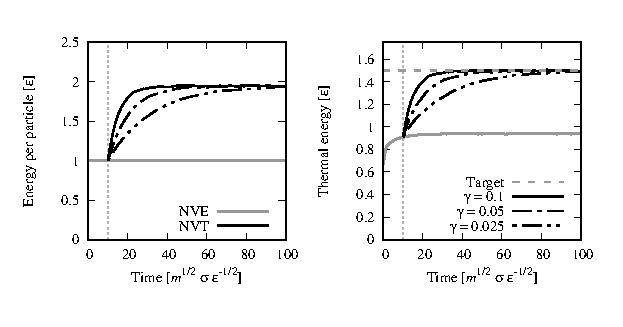
\includegraphics[width = \textwidth]{figures/Langevin.eps}
  \end{center}
  \caption{\label{Langevin}Average energy per particle (\textit{left}) and 
           thermal energy (\textit{right}) for a system of $10^5$ particles
           with Lennard-Jones interactions in a $128^3\ \sigma^3$ box with
           periodic boundary conditions. The solid grey line corresponds to an 
           NVE simulation, while the black curves plot the evolution of a 
           thermostatted system with different values of the friction parameter 
           $\gamma$. The latter simulations begin from the NVE state at
           $t = 10$.}
\end{figure}

The solid grey lines in Figure \ref{Langevin} follow the evolution of the mean 
energy per particle and the thermal energy for an NVE simulation (constant 
number of particles, volume and energy) of particles with Lennard-Jones 
interactions. At the time marked by the vertical dotted line, I saved the state 
of the system and used it to set up several thermostatted simulations with a 
target thermal energy marked by the horizontal dashed grey line. As you can see, 
the NVE algorithm keeps the mean energy per particle constant, but the NVT 
alternative introduced here allows it to change. Furthermore, you'll notice that 
smaller values of the friction constant $\gamma$ lead to longer relaxation 
times.


\begin{comment}
\begin{lstlisting}
%! codefile: code/Langevin.cu
%! codeinsert: includeGenericMD
%! codeinsert: includeLennard-Jones
%! codeinsert: includeVerletNVT

%! codeinsert: namespaceUAMMD

struct InputParameters {
  %! codeinsert: genericMDInputParameters
  %! codeinsert: Lennard-JonesInputParameters
  %! codeinsert: LangevinParameters
  real mass;
  %! codeinsert: checkpointParameters
};

InputParameters readParameterFile(std::shared_ptr<System> sys)
{
  if(!std::ifstream("data.main").good()) {
    sys->log<System::WARNING>("File data.main not found. Creating file with default values.");
    std::ofstream defaultParameters("data.main");
    if(not defaultParameters.is_open()) {
      sys->log<System::CRITICAL>("Unable to create data.main file. Halting program.");
      exit(-1);
    }
    %! codeinsert: genericMDDefaultParameterList
    %! codeinsert: Lennard-JonesDefaultParameterList
    %! codeinsert: LangevinDefaultParameterList
    defaultParameters<<"mass 1.0"<<endl;
  }
  InputFile parameterFile("data.main", sys);
  InputParameters params;

  %! codeinsert: genericMDReadParameterFile
  %! codeinsert: Lennard-JonesReadParameterFile
  %! codeinsert: LangevinReadParameterFile
  %! codeinsert: checkpointReadParameterFile
  parameterFile.getOption("mass",
    InputFile::Required)>>params.mass;

  return params;
}

%! codeinsert: getTotalEnergy

%! codeinsert: getTotalMomentum

%! codeinsert: getThermalEnergy

int main(int argc, char *argv[]){

  auto sys = make_shared<System>(argc, argv);

  %! codeinsert: loadParameters src: chapters/first_simulation.tex

  int numberOfParticles = simParams.numberOfParticles;
  auto particles
    = make_shared<ParticleData>(numberOfParticles, sys);

  real L = simParams.L;

  %! codeinsert: LJsimulationBox src: chapters/first_simulation.tex

  %! codeinsert: checkpointInitialPositions

  %! codeinsert: Lennard-JonesFillMass

  %! codeinsert: VerletNVTParameters

  if(simParams.inputFile.empty()) {
    sys->log<System::MESSAGE>("UAMMD will generate new velocities.");
    VerletParams.initVelocities = true;
  } else {
    VerletParams.initVelocities = false;
  }

  %! codeinsert: Verlet src: chapters/first_simulation.tex

  %! codeinsert: Lennard-JonesPotential

  %! codeinsert: Lennard-JonesInteraction src: chapters/first_simulation.tex

  %! codeinsert: Lennard-JonesOutputFiles

  int numberOfSteps = simParams.numberOfSteps;
  int printEverynSteps = simParams.printEverynSteps;

  for(int step = 0; step < numberOfSteps; ++step) {
    integrator->forwardTime();

    %! codeinsert: Lennard-JonesOutputData

    %! codeinsert: saveState
  }

  sys->finish();

  return 0;
}
%! codeend
\end{lstlisting}
\end{comment}

\section{Brownian dynamics}

Observed through a microscope, a small grain of pollen floating in water jiggles 
incessantly due to impacts from the even tinier molecules that surround it. In 
the grain's minuscule world, no sooner has it started to move one way than it 
feels a sudden jolt that directs it somewhere else. The resulting overdamped 
dynamics may conveniently be thought of as a succession of small random jumps in 
which the velocity plays no role.

In mathematical terms, we express the evolution of the system with a stochastic 
differential equation (in the It\=o interpretation).
\begin{equation*}
  d\mathbf{r} = M\mathbf{F}\ dt + \sqrt{2 M k_BT} \mathbf{dW}.
\end{equation*}
Here, $\mathbf{r}$ represents the position and $\mathbf{F}$ the force. $M$ is 
known as the mobility and $\mathbf{dW}$ stands for the Wiener process. We won't 
worry about the mathematical subtleties and will simply accept that the 
equation, known as Brownian motion, adequately models small immersed particles, 
like fine dust, for example.

Brownian dynamics have counter-intuitive properties. Because the particles 
change the direction of their displacements from one instant to the next, we 
cannot define the velocities, the microscopic environment lacks inertia, and 
mass ceases to play a role in the motions.

UAMMD includes several integrators for the aforementioned stochastic 
differential equation, the most popular of which is the Euler-Maruyama scheme.
Include them with:
\begin{lstlisting}
%! codeblock: includeBrownianDynamics
# include "Integrator/BrownianDynamics.cuh" //!
%! codeblockend !//
\end{lstlisting}

The new integrators need a thermal energy and viscosity parameter, as well as 
the particle radius. The latter two values determine the mobility. Larger 
particles and higher viscosities lead to smaller mobilities.
\begin{lstlisting}
%! codeblock: BrownianDynamicsInputParameters
  real thermalEnergy;
  real viscosity;
  real hydrodynamicRadius; //!
%! codeblockend !//
\end{lstlisting}
We will list them as having a default value equal to one,
\begin{lstlisting}
%! codeblock: BrownianDynamicsDefaultParameterList
    defaultParameters<<"thermalEnergy 1.0"<<endl;
    defaultParameters<<"viscosity 1.0"<<endl;
    defaultParameters<<"hydrodynamicRadius 1.0"<<endl; //!
%! codeblockend !//
\end{lstlisting}
and will read them in from the \texttt{data.main} parameter file in the 
customary way.
\begin{comment}
\begin{lstlisting}
%! codeblock: BrownianDynamicsReadParameterFile
  parameterFile.getOption("thermalEnergy",
    InputFile::Required)>>params.thermalEnergy;
  parameterFile.getOption("viscosity",
    InputFile::Required)>>params.viscosity;
  parameterFile.getOption("hydrodynamicRadius",
    InputFile::Required)>>params.hydrodynamicRadius; //!
%! codeblockend !//
\end{lstlisting}
\end{comment}

When we read the initial configuration from a file, it should only contain 
coordinates, not velocities.
\begin{lstlisting}
%! codeblock: BrownianDynamicsReadPosition
    auto position
      = particles->getPos(access::location::cpu,
                          access::mode::write);

    std::string inputFile = simParams.inputFile;
    std::ifstream in(inputFile);

    for(int i = 0; i < numberOfParticles; ++i) {
      in>>position[i].x>>position[i].y>>position[i].z;
      position[i].w = 0;
    }
%! codeblockend
\end{lstlisting}

Activate Brownian dynamics integrators with the pattern that we have become 
accustomed to by now.
\begin{lstlisting}
%! codeblock: BrownianDynamicsIntegrator
  using EulerMaruyama = BD::EulerMaruyama;
  EulerMaruyama::Parameters EMParams;
  EMParams.dt = simParams.dt;
  EMParams.temperature = simParams.thermalEnergy;
  EMParams.viscosity = simParams.viscosity;
  EMParams.hydrodynamicRadius = simParams.hydrodynamicRadius;

  auto integrator
    = make_shared<EulerMaruyama>(particles, sys, EMParams);//!
%! codeblockend !//
\end{lstlisting}
In previous Lennard-Jones simulations, we got away with a time step of $10^{-2}$ 
but this setup really requires safer steps of size $10^{-3}$, as random 
fluctuations could push two particles too close together and this might create 
an explosive chain reaction.

In many ways, however, Brownian Dynamics simplifies our work. We no longer have 
to deal with masses and we don't need the velocities to restore the state. 
Momentum has become an undefined property and we can output the temperature 
directly, without having to calculate it first.
\begin{lstlisting}
%! codeblock: BrownianDynamicsOutputMacro
      macro<<step*simParams.dt<<" ";
      macro<<getTotalEnergy(integrator, particles)<<" ";
      macro<<" N/A N/A N/A "; /* Undefined total momentum */
      macro<<simParams.thermalEnergy<<endl; //!
%! codeblockend !//
\end{lstlisting}

\begin{comment}
%! codeblock: genericBDDefaultParameterList
    defaultParameters<<"numberOfParticles 100000"<<endl;
    defaultParameters<<"boxSize 128"<<endl;
    defaultParameters<<"timeStep 0.001"<<endl;
    defaultParameters<<"outputFile Lennard-Jones.dat"<<endl;
    defaultParameters<<"measurementsFile LJmacro.dat"<<endl;
    defaultParameters<<"numberOfSteps 10000"<<endl;
    defaultParameters<<"printEverynSteps 1000"<<endl;
%! codeblockend


\begin{lstlisting}
%! codefile: code/BrownianDynamics.cu
%! codeinsert: includeGenericMD
%! codeinsert: includeLennard-Jones
%! codeinsert: includeBrownianDynamics

%! codeinsert: namespaceUAMMD

struct InputParameters {
  %! codeinsert: genericMDInputParameters
  %! codeinsert: Lennard-JonesInputParameters
  %! codeinsert: BrownianDynamicsInputParameters
  std::string inputFile;
};

InputParameters readParameterFile(std::shared_ptr<System> sys)
{
  if(!std::ifstream("data.main").good()) {
    sys->log<System::WARNING>("File data.main not found. Creating file with default values.");
    std::ofstream defaultParameters("data.main");
    if(not defaultParameters.is_open()) {
      sys->log<System::CRITICAL>("Unable to create data.main file. Halting program.");
      exit(-1);
    }
    %! codeinsert: genericBDDefaultParameterList
    %! codeinsert: Lennard-JonesDefaultParameterList
    %! codeinsert: BrownianDynamicsDefaultParameterList
  }
  InputFile parameterFile("data.main", sys);
  InputParameters params;

  %! codeinsert: genericMDReadParameterFile
  %! codeinsert: Lennard-JonesReadParameterFile
  %! codeinsert: BrownianDynamicsReadParameterFile
  parameterFile.getOption("inputFile",
    InputFile::Optional)>>params.inputFile;

  return params;
}

%! codeinsert: getTotalEnergy

int main(int argc, char *argv[]){

  auto sys = make_shared<System>(argc, argv);

  %! codeinsert: loadParameters src: chapters/first_simulation.tex

  int numberOfParticles = simParams.numberOfParticles;
  auto particles
    = make_shared<ParticleData>(numberOfParticles, sys);

  real L = simParams.L;

  %! codeinsert: LJsimulationBox src: chapters/first_simulation.tex

  if(simParams.inputFile.empty()) {
    sys->log<System::MESSAGE>("Creating new initial positions.");

    auto position
      = particles->getPos(access::location::cpu,
                          access::mode::write);

    auto initial =  initLattice(box.boxSize,
                                numberOfParticles, sc);

    std::copy(initial.begin(), initial.end(), position.begin());
  } else {
    sys->log<System::MESSAGE>("Reading initial positions and velocities from file.");
    %! codeinsert: BrownianDynamicsReadPosition
  }

  %! codeinsert: BrownianDynamicsIntegrator

  %! codeinsert: Lennard-JonesPotential

  %! codeinsert: Lennard-JonesInteraction src: chapters/first_simulation.tex

  %! codeinsert: Lennard-JonesOutputFiles

  int numberOfSteps = simParams.numberOfSteps;
  int printEverynSteps = simParams.printEverynSteps;

  for(int step = 0; step < numberOfSteps; ++step) {
    integrator->forwardTime();

    if(printEverynSteps > 0
       and step % printEverynSteps == 1) {

      auto position
        = particles->getPos(access::location::cpu,
                            access::mode::read);
      const int * index = particles->getIdOrderedIndices(access::location::cpu);

      out<<endl;
      for(int id = 0; id < numberOfParticles; ++id)
        out<<box.apply_pbc(make_real3(position[index[id]]))<<endl;

      %! codeinsert: BrownianDynamicsOutputMacro
    }
  }

  sys->finish();

  return 0;
}
%! codeend
\end{lstlisting}
\end{comment}

The Brownian dynamics integrator has an interesting additional feature. You can 
specify the elements of a strain-rate tensor $K$ that will deform the fluid 
around your suspended particles, dragging them along. In that case, the 
algorithm will solve the equation
\begin{equation*}
  d\mathbf{r} = (K\mathbf{r} + M\mathbf{F})\ dt + \sqrt{2 M k_BT} \mathbf{dW}.
\end{equation*}

As an example, we can change a few things in the Brownian dynamics code above to 
simulate suspended particles in a simple shear flow, where the velocity in the 
$y$ direction depends linearly on the $z$ coordinate. I trust that by now you 
know how to add the new shear rate parameter to the module. A good default value 
might be
\begin{lstlisting}
    defaultParameters<<"shearRate 0.01"<<endl;
\end{lstlisting}
We'll let our simulation box extend outwards indefinitely to avoid the problems 
that periodic boundary conditions would cause. We do not want particles leaving 
the top of our box and ramming into periodic images that oppose the flow.
\begin{lstlisting}
%! codeblock: infiniteL
  real L = std::numeric_limits<real>::infinity(); //!
%! codeblockend !//
\end{lstlisting}
But careful! Remember that we used the box size to lay out the particles on a 
lattice, so change the initial positions to
\begin{lstlisting}
%! codeblock: shearInitialPositions
    auto initial
      =  initLattice(make_real3(simParams.L, simParams.L,
                                simParams.L),
                     numberOfParticles, sc); //!
%! codeblockend !//
\end{lstlisting}
Periodic boundary conditions will no longer work, so we'll output the positions 
directly.
\begin{lstlisting}
%! codeblock: shearOutputPositions
        out<<make_real3(position[index[id]])<<endl; //!
%! codeblockend !//
\end{lstlisting}

UAMMD stores the strain-rate tensor $K$ as a vector of three \texttt{real3} 
variables. \texttt{K[0]} represents the first row of components,
$(k_{xx},\ k_{xy},\ k_{xz})$ and
\begin{lstlisting}
%! codeblock: setShearRate
  EMParams.K[1].z = simParams.shearRate; //!
%! codeblockend !//
\end{lstlisting}
would set the value of the $k_{yz}$ component. The default value for all 
components is zero.

\begin{comment}
\begin{lstlisting}
%! codefile: code/shear.cu
%! codeinsert: includeGenericMD
%! codeinsert: includeLennard-Jones
%! codeinsert: includeBrownianDynamics

%! codeinsert: namespaceUAMMD

struct InputParameters {
  %! codeinsert: genericMDInputParameters
  %! codeinsert: Lennard-JonesInputParameters
  %! codeinsert: BrownianDynamicsInputParameters
  real shearRate;
  std::string inputFile;
};

InputParameters readParameterFile(std::shared_ptr<System> sys)
{
  if(!std::ifstream("data.main").good()) {
    sys->log<System::WARNING>("File data.main not found. Creating file with default values.");
    std::ofstream defaultParameters("data.main");
    if(not defaultParameters.is_open()) {
      sys->log<System::CRITICAL>("Unable to create data.main file. Halting program.");
      exit(-1);
    }
    %! codeinsert: genericBDDefaultParameterList
    %! codeinsert: Lennard-JonesDefaultParameterList
    %! codeinsert: BrownianDynamicsDefaultParameterList
    defaultParameters<<"shearRate 0.01"<<endl;
  }
  InputFile parameterFile("data.main", sys);
  InputParameters params;

  %! codeinsert: genericMDReadParameterFile
  %! codeinsert: Lennard-JonesReadParameterFile
  %! codeinsert: BrownianDynamicsReadParameterFile
  parameterFile.getOption("inputFile",
    InputFile::Optional)>>params.inputFile;
  params.shearRate = 0;
  parameterFile.getOption("shearRate",
    InputFile::Optional)>>params.shearRate;

  return params;
}

%! codeinsert: getTotalEnergy

int main(int argc, char *argv[]){

  auto sys = make_shared<System>(argc, argv);

  %! codeinsert: loadParameters src: chapters/first_simulation.tex

  int numberOfParticles = simParams.numberOfParticles;
  auto particles
    = make_shared<ParticleData>(numberOfParticles, sys);

  %! codeinsert: infiniteL

  %! codeinsert: LJsimulationBox src: chapters/first_simulation.tex

  if(simParams.inputFile.empty()) {
    sys->log<System::MESSAGE>("Creating new initial positions.");

    auto position
      = particles->getPos(access::location::cpu,
                          access::mode::write);

    %! codeinsert: shearInitialPositions

    std::copy(initial.begin(), initial.end(), position.begin());
  } else {
    sys->log<System::MESSAGE>("Reading initial positions and velocities from file.");
    %! codeinsert: BrownianDynamicsReadPosition
  }

  using EulerMaruyama = BD::EulerMaruyama;
  EulerMaruyama::Parameters EMParams;
  EMParams.dt = simParams.dt;
  EMParams.temperature = simParams.thermalEnergy;
  EMParams.viscosity = simParams.viscosity;
  EMParams.hydrodynamicRadius = simParams.hydrodynamicRadius;
  %! codeinsert: setShearRate

  auto integrator
    = make_shared<EulerMaruyama>(particles, sys, EMParams);//!

  %! codeinsert: Lennard-JonesPotential

  %! codeinsert: Lennard-JonesInteraction src: chapters/first_simulation.tex

  %! codeinsert: Lennard-JonesOutputFiles

  int numberOfSteps = simParams.numberOfSteps;
  int printEverynSteps = simParams.printEverynSteps;

  for(int step = 0; step < numberOfSteps; ++step) {
    integrator->forwardTime();

    if(printEverynSteps > 0
       and step % printEverynSteps == 1) {

      auto position
        = particles->getPos(access::location::cpu,
                            access::mode::read);
      const int * index = particles->getIdOrderedIndices(access::location::cpu);

      out<<endl;
      for(int id = 0; id < numberOfParticles; ++id)
        %! codeinsert: shearOutputPositions

      %! codeinsert: BrownianDynamicsOutputMacro
    }
  }

  sys->finish();

  return 0;
}
%! codeend
\end{lstlisting}
\end{comment}

\section{Custom integrators}

You would like your code to do something different. Of course you would. As soon 
as you learn the basics, you start imagining scenarios with two thermostats 
driving heat flow, or sinks and sources of particles. Then you need to write 
your own integrator, implementing your custom versions of the 
\texttt{forwardTime} and \texttt{sumEnergy} methods.

As a simple educational exersice, we'll develop an Andersen thermostat for 
UAMMD. The idea behind the algorithm resembles that of the Langevin thermostat. 
Our system interacts with a medium at temperature $T$ that we do not represent 
explicitly. In contrast to the Langevin method, where the thermal fluctuations 
affect every time step, our particles only occasionally crash into a particle in 
the medium and acquire a new velocity. In the time between collisions, 
characterised by the \textit{mean free time}, they obey the laws of Hamiltonian 
mechanics. Hence, our Andersen integrator will incorporate two extra parameters. 
\begin{lstlisting}
%! codeblock: AndersenParameters
  real thermalEnergy;
  real meanFreeTime; //!
%! codeblockend !//
\end{lstlisting}
Don't forget to set their default values and read them in from 
\texttt{data.main}. Within the main function, instead of \texttt{VerletNVE}, we 
will use 
\texttt{Andersen}.
\begin{lstlisting}
%! codeblock: VerletAndersen
  using Verlet = Andersen; //!
%! codeblockend !//
\end{lstlisting}
We will construct the integrator adding the two new parameters into the mix.
\begin{lstlisting}
%! codeblock: Andersen
  auto integrator
    = make_shared<Verlet>(particles, sys, VerletParams,
                          simParams.thermalEnergy,
                          simParams.meanFreeTime); //!
%! codeblockend !//
\end{lstlisting}
Simple enough to use, but the Andersen thermostat does not exist yet, so we will 
have to code it ourselves.

Let me begin with the heart of the algorithm. Particles have a given probability 
of interacting with the medium and changing their velocity. Because we can 
determine the outcome of this process independently for each of the particles, 
the function becomes an ideal candidate for parallelisation. We will therefore 
write the \texttt{thermalise} function as \texttt{\_\_global\_\_}, that is to 
say, the operations will run on the GPU, but we will call them directly from a 
host function running on the CPU.

We want each thread to apply to a different particle. Thread number $i$ will 
operate on particle $i$. Therefore, if $i$ exceeds the number of particles, we 
just return without doing anything.
\begin{lstlisting}
%! codeblock: AndersenThermalise
__global__ void thermalise(int N,
                           real3 * velocity,
                           real * mass,
                           real thermalEnergy,
                           real probability,
                           uint counter,
                           uint seed){
  const int i = blockIdx.x*blockDim.x + threadIdx.x;
  if(i > N) return; //!
  %! codeinsert: SaruPRNG
  %! codeinsert: thermalVelocity
%! codeblockend !//
\end{lstlisting}
We need independent random numbers among different threads and time steps. UAMMD 
includes the Saru generator, which accepts three seeds. Using the thread number 
and a time step counter gets us the desired independent numbers.
\begin{lstlisting}
%! codeblock: SaruPRNG
  Saru rng(i, counter, seed); //!
%! codeblockend !//
\end{lstlisting}
Saru outputs a uniformly distributed random number in the $[0,\ 1)$ interval 
with \texttt{rng.f()}. If it turns out that the particle interacted with the 
medium, then we replace its velocity. With \texttt{rng.gf(mean, std)} you create 
two random numbers from a normal distribution with the specified mean and 
standard deviation. Because we need three components, we call \texttt{rng.gf} 
twice, but the second time we only keep one of the two numbers generated 
(selected with the \texttt{.x}). That will close the parallel section of our 
algorithm.
\begin{lstlisting}
%! codeblock: thermalVelocity
  if(rng.f() < probability) {
    real velocitystd = sqrtf(thermalEnergy/mass[i]);
    velocity[i] = make_real3(rng.gf(0, velocitystd),
                             rng.gf(0, velocitystd).x);
  }

  return;
} //!
%! codeblockend !//
\end{lstlisting}

Now we can write the Andersen integrator. It should behave just like 
\texttt{VerletNVE}, but call the \texttt{thermalise} function at the end of 
every time step. We \textit{could} copy the whole of \texttt{VerletNVE},
changing its name and tweaking its behaviour, but that would make our example 
unnecesarily long. Instead, we shall write an integrator that inherits from
\texttt{VerletNVE}, and that will save us from repeating most of its content.
\begin{lstlisting}
%! codeblock: AndersenThermostat
class Andersen: public VerletNVE {
  uint seed;
  real thermalEnergy;
  real meanFreeTime;
  real dt;

  public: //!
  %! codeinsert: AndersenConstructor
  %! codeinsert: AndersenForwardTime
%! codeblockend !//
\end{lstlisting}
Above, \texttt{seed} stands for the random number generator seed.

In addition to pointers to the \texttt{ParticleData} and \texttt{System}, we 
agreed that the constructor would take the thermal energy and mean free time as 
parameters. Before it initialises its internal \texttt{dt} and \texttt{seed} 
variables, it calls the \texttt{VerletNVE} constructor and sets the values of
\texttt{thermalEnergy} and \texttt{meanFreeTime}.
\begin{lstlisting}
%! codeblock: AndersenConstructor
    Andersen(std::shared_ptr<ParticleData> particles,
             std::shared_ptr<System> sys,
             Parameters params,
             real i_thermalEnergy,
             real i_meanFreeTime) :
             VerletNVE(particles, sys, params),
             thermalEnergy(i_thermalEnergy),
             meanFreeTime(i_meanFreeTime){
      dt = params.dt;
      seed = sys->rng().next32();
    } //!
%! codeblockend !//
\end{lstlisting}

The Andersen \texttt{forwardTime} function simply calls the parent 
\texttt{VerletNVE} version and then calls \texttt{thermalise}. The code in 
between sets up the values of all the arguments in the latter call. Within UAMMD
integrators, the variables \texttt{sys} and \texttt{pd} store the pointers to 
the \texttt{System} and \texttt{ParticleData} information.
\begin{lstlisting}
%! codeblock: AndersenForwardTime
    virtual void forwardTime() override{
      VerletNVE::forwardTime();

      real collisionProbability
        = dt/meanFreeTime;

      auto particles = pd;
      auto velocity
        = particles->getVel(access::location::gpu,
                            access::mode::readwrite);
      auto mass
        = particles->getMass(access::location::gpu,
                             access::mode::readwrite);

      static uint numberOfCalls = 0;
      int numberOfParticles = particles->getNumParticles();
      int Nthreads = 128;
      int Nblocks = numberOfParticles/Nthreads
                    + ((numberOfParticles%Nthreads)?1:0);

      numberOfCalls++;
      thermalise<<<Nblocks,Nthreads,0,0>>>(numberOfParticles,
                                           velocity.raw(),
                                           mass.raw(),
                                           thermalEnergy,
                                           collisionProbability,
                                           numberOfCalls,
                                           seed);
    }
}; //!
%! codeblockend !//
\end{lstlisting}
We won't have to write \texttt{sumEnergy} because we inherited the parent 
version of the function, which we don't need to change.

I copied the definition of the Andersen thermostat above my \texttt{main} 
function, as I prefer to keep each example in its own file, but the standard 
practice would have it in a separate file, which you could then include at the 
beginning of your module.

\begin{comment}
\begin{lstlisting}
%! codefile: code/Andersen.cu
%! codeinsert: includeGenericMD
%! codeinsert: includeLennard-Jones
# include "Integrator/VerletNVE.cuh"

%! codeinsert: namespaceUAMMD

struct InputParameters {
  %! codeinsert: NVEInputParameters
  %! codeinsert: checkpointParameters
  %! codeinsert: AndersenParameters
};

InputParameters readParameterFile(std::shared_ptr<System> sys)
{
  if(!std::ifstream("data.main").good()) {
    sys->log<System::WARNING>("File data.main not found. Creating file with default values.");
    std::ofstream defaultParameters("data.main");
    if(not defaultParameters.is_open()) {
      sys->log<System::CRITICAL>("Unable to create data.main file. Halting program.");
      exit(-1);
    }
    %! codeinsert: NVEDefaultParameterList
    defaultParameters<<"thermalEnergy 1.0"<<endl;
    defaultParameters<<"meanFreeTime 1.0"<<endl;
  }
  InputFile parameterFile("data.main", sys);
  InputParameters params;

  %! codeinsert: NVEReadParameterFile
  %! codeinsert: checkpointReadParameterFile
  parameterFile.getOption("thermalEnergy",
    InputFile::Required)>>params.thermalEnergy;
  parameterFile.getOption("meanFreeTime",
    InputFile::Required)>>params.meanFreeTime;

  return params;
}

%! codeinsert: getTotalEnergy

%! codeinsert: getTotalMomentum

%! codeinsert: getThermalEnergy

%! codeinsert: AndersenThermalise

%! codeinsert: AndersenThermostat

int main(int argc, char *argv[]){

  auto sys = make_shared<System>(argc, argv);

  %! codeinsert: loadParameters src: chapters/first_simulation.tex

  int numberOfParticles = simParams.numberOfParticles;
  auto particles
    = make_shared<ParticleData>(numberOfParticles, sys);

  real L = simParams.L;

  %! codeinsert: LJsimulationBox src: chapters/first_simulation.tex

  %! codeinsert: checkpointInitialPositions

  %! codeinsert: Lennard-JonesFillMass

  %! codeinsert: VerletAndersen
  Verlet::Parameters VerletParams;
  VerletParams.dt = simParams.dt;
  %! codeinsert: checkpointInitVelocities

  %! codeinsert: Andersen

  %! codeinsert: Lennard-JonesPotential

  %! codeinsert: Lennard-JonesInteraction src: chapters/first_simulation.tex

  %! codeinsert: Lennard-JonesOutputFiles

  int numberOfSteps = simParams.numberOfSteps;
  int printEverynSteps = simParams.printEverynSteps;

  for(int step = 0; step < numberOfSteps; ++step) {
    integrator->forwardTime();

    %! codeinsert: Lennard-JonesOutputData

    %! codeinsert: saveState
  }

  sys->finish();

  return 0;
}
%! codeend
\end{lstlisting}
\end{comment}

You might feel let down by the example above. I chose the Andersen thermostat 
precisely because I could sidestep the problem of dealing with all the 
interactions. Having familiarised ourselves with the inner workings of an 
interactor, we can boldly proceed to write a complete integrator from scratch. 
The Euler scheme probably constitutes the simplest interesting example.

Here comes a parallel version of the rule for updating positions and velocities.
\begin{lstlisting}
%! codeblock: EulerStep
__global__ void EulerStep(int N, real dt,
                          real4 * position,
                          real3 * velocity,
                          real * mass,
                          real4 * force){
  const int i = blockIdx.x*blockDim.x + threadIdx.x;
  if(i > N) return;

  position[i] += make_real4(velocity[i]*dt, real(0.0));
  velocity[i] += make_real3(force[i].x*dt/mass[i],
                            force[i].y*dt/mass[i],
                            force[i].z*dt/mass[i]);

  return;
} //!
%! codeblockend !//
\end{lstlisting}
Integrators do not just move the system forward in time. They also calculate the 
kinetic part of the energy. The short function that follows adds the kinetic 
energy of each particle to the energy vector (in parallel).
\begin{lstlisting}
%! codeblock: kineticEnergy
__global__ void kineticEnergy(int N,
                              real3 * velocity,
                              real * mass,
                              real * energy){
  const int i = blockIdx.x*blockDim.x + threadIdx.x;
  if(i > N) return;

  energy[i] += real(0.5)*mass[i]*dot(velocity[i], velocity[i]);

  return;
} //!
%! codeblockend !//
\end{lstlisting}

As with the Andersen thermostat, we will have to write an \texttt{Integrator}. 
This includes a constructor and the \texttt{forwardTime} and \texttt{sumEnergy} 
methods. The constructor will just set the value of the time step and call the 
parent constructor for \texttt{Integrator}.
\begin{lstlisting}
%! codeblock: Euler
class Euler : public Integrator {
  real dt;

  public:
    struct Parameters {
      real dt;
    };

    Euler(std::shared_ptr<ParticleData> particles,
          std::shared_ptr<System> sys,
          Parameters params) :
          Integrator(particles,
                     std::make_shared<ParticleGroup>(particles, sys, "ALL"),
                     sys, "Euler"),
          dt(params.dt){} //!
  %! codeinsert: EulerForwardTime
  %! codeinsert: EulerSumEnergy
%! codeblockend !//
\end{lstlisting}
To move forward in time, we will calculate the forces on every particle. 
Therefore, we first clear the force vector.
\begin{lstlisting}
%! codeblock: EulerForwardTime
    virtual void forwardTime() override{
      auto particles = pd;

      {
        auto force
          = particles->getForce(access::location::cpu,
                                access::mode::write);

        std::fill(force.begin(), force.end(),
                  make_real4(0.0, 0.0, 0.0, 0.0));
      } //!
      %! codeinsert: EulerSumForces
      %! codeinsert: callEulerStep
%! codeblockend !//
\end{lstlisting}
Next, we use the following loop to run the \texttt{sumForce} method of every 
interaction added to the integrator.
\begin{lstlisting}
%! codeblock: EulerSumForces
      for(auto interaction: interactors) {
        interaction->sumForce();
      } //!
%! codeblockend !//
\end{lstlisting}
We close \texttt{forwardTime} getting the references to the position, velocity, 
mass and force vectors ready for calling \texttt{EulerStep}.
\begin{lstlisting}
%! codeblock: callEulerStep
      auto position
        = particles->getPos(access::location::gpu,
                            access::mode::readwrite);

      auto velocity
        = particles->getVel(access::location::gpu,
                            access::mode::readwrite);

      auto mass
        = particles->getMass(access::location::gpu,
                             access::mode::read);

      auto force
        = particles->getForce(access::location::gpu,
                              access::mode::read);

      int numberOfParticles = particles->getNumParticles();
      int Nthreads = 128;
      int Nblocks = numberOfParticles/Nthreads
                    + ((numberOfParticles%Nthreads)?1:0);

      EulerStep<<<Nblocks,Nthreads,0,0>>>(numberOfParticles, dt,
                                          position.raw(),
                                          velocity.raw(),
                                          mass.raw(),
                                          force.raw());
    } //!
%! codeblockend !//
\end{lstlisting}

Similarly, the final \texttt{sumEnergy} function in the Euler 
\texttt{Integrator} just prepares the vectors for a call to 
\texttt{kineticEnergy}.
\begin{lstlisting}
%! codeblock: EulerSumEnergy
    virtual real sumEnergy() override{
      auto particles = pd;

      auto velocity
        = particles->getVel(access::location::gpu,
                            access::mode::read);

      auto mass
        = particles->getMass(access::location::gpu,
                             access::mode::read);

      auto energy
        = particles->getEnergy(access::location::gpu,
                               access::mode::write);

      int numberOfParticles = particles->getNumParticles();
      int Nthreads = 128;
      int Nblocks = numberOfParticles/Nthreads
                    + ((numberOfParticles%Nthreads)?1:0);

      kineticEnergy<<<Nblocks,Nthreads,0,0>>>(numberOfParticles,
                                              velocity.raw(),
                                              mass.raw(),
                                              energy.raw());
      return 0;
    }
}; //!
%! codeblockend !//
\end{lstlisting}

In our attempt to keep things as simple as possible, we have omitted the code 
that initialises velocities. You will have to deal with these yourself either by 
setting them up within \texttt{main} or extending the \texttt{Integrator} with 
code that you could copy from \texttt{VerletNVE}.

Perhaps you would enjoy comparing simulations carried out with Verlet and Euler 
integrations. If so, I recommend you compare the evolution of the total energy 
of the system. You should see an unreasonable drift in the energy for the Euler 
scheme which explains why researchers generally prefer Verlet's method.

\begin{comment}
How to instantiate the Euler integrator:
\begin{lstlisting}
%! codeblock: EulerIntegrator
  Euler::Parameters simParams;
  simParams.dt = 0.001;

  auto integrator
    = make_shared<Euler>(particles, sys, simParams); //!
%! codeblockend !//
\end{lstlisting}

Euler does not implement initalising velocities, hence the following block.
\begin{lstlisting}
%! codeblock: EulerInitialConditions
  {
    auto velocity
      = particles->getVel(access::location::cpu,
                          access::mode::write);

    for(int i = 0; i < numberOfParticles; ++i) {
      velocity[i] = make_real3(sys->rng().gaussian(0,1),
                               sys->rng().gaussian(0,1),
                               sys->rng().gaussian(0,1));
    }
  }

  {
    auto mass
      = particles->getMass(access::location::cpu,
                           access::mode::write);

    std::fill(mass.begin(), mass.end(), real(1.0));
  } //!
%! codeblockend !//
\end{lstlisting}

One way to integrate the Euler scheme into a UAMMD module follows.
\begin{lstlisting}
%! codefile: code/Euler.cu
# include "uammd.cuh"
# include "utils/InitialConditions.cuh"
# include "Interactor/Potential/Potential.cuh"
# include "Interactor/NeighbourList/CellList.cuh"
# include "Interactor/PairForces.cuh"
# include "Integrator/Integrator.cuh"

using namespace uammd;
using std::make_shared;
using std::endl;

%! codeinsert: getTotalEnergy

%! codeinsert: getTotalMomentum

%! codeinsert: getThermalEnergy

%! codeinsert: EulerStep

%! codeinsert: kineticEnergy

%! codeinsert: Euler

int main(int argc, char *argv[]){

  auto sys = make_shared<System>(argc, argv);

  %! codeinsert: particleData src: chapters/first_simulation.tex

  %! codeinsert: latticeInitialConditions src: chapters/first_simulation.tex

  %! codeinsert: EulerInitialConditions

  %! codeinsert: EulerIntegrator

  %! codeinsert: Lennard-JonesPotential src: chapters/first_simulation.tex

  %! codeinsert: Lennard-JonesInteraction src: chapters/first_simulation.tex

  std::string outputFile = "Lennard-Jones.dat";
  std::ofstream out(outputFile);
  std::string macroFile = "LJmacro.dat";
  std::ofstream macro(macroFile);

  int numberOfSteps = 1000;
  int printEverynSteps = 100;

  for(int step = 0; step < numberOfSteps; ++step) {
    integrator->forwardTime();

    %! codeinsert: Lennard-JonesOutputData
  }

  sys->finish();

  return 0;
} //!
%! codeend !//
\end{lstlisting}
\end{comment}

\section{Structure and dynamics}

Returning to the issue of measuring, I would like to write a short function to 
determine the density of a system at different heights of the $z$ coordinate. It 
will need to know the simulation box cross section, the number of particles and 
the list of positions. To calculate the density, we simply slice our system 
into bins, count the number of particles in each bin, and divide this number by 
the volume corresponding to each slice. We'll allow the user to specify the name 
of an output file, the lower and upper limits, and the number of bins into which 
the data will be grouped.
\begin{lstlisting}
%! codeblock: density
void density(std::string filename, real crossSection,
             int numberOfParticles, real4 * position,
             real min, real max, int numberOfBins){ //!
%! codeblockend !//
\end{lstlisting} 
We don't want each new measurement to overwrite the previous one, so we specify 
that we will append new data (\texttt{std::ios\_base::app}). Next, we work out 
the bin size and clear the list of bins.
\begin{lstlisting}
%! codeblock: densityPrepareBins
  std::ofstream densityFile;
  densityFile.open(filename, std::ios_base::app);

  real binSize = (max - min)/numberOfBins;
  static std::vector<real> bin;
  bin.resize(numberOfParticles);
  std::fill(bin.begin(), bin.end(), real(0.0)); //!
%! codeblockend !//
\end{lstlisting}
For each particle, add one to its corresponding bin.
\begin{lstlisting}
%! codeblock: densityFillBins
  for(int i = 0; i < numberOfParticles; ++i) {
    int binNumber = (int) floorf((position[i].z - min)/binSize);

    if(binNumber >= 0 and binNumber < numberOfBins) {
      bin[binNumber]++;
    }
  } //!
%! codeblockend !//
\end{lstlisting}
Finally, output the positions and their corresponding densities.
\begin{lstlisting}
%! codeblock: densityOutput
  for(int i = 0; i < numberOfBins; ++i) {
    densityFile<<min + (i + real(0.5))*binSize<<" "
               <<bin[i]/(numberOfParticles*binSize*crossSection)
               <<endl;
  }
  densityFile<<endl;
} //!
%! codeblockend !//
\end{lstlisting}
I tested the function by including it into the free expansion of an ideal gas 
that we saw in chapter one, and I plotted the result in Figure \ref{density}.

\begin{figure}
  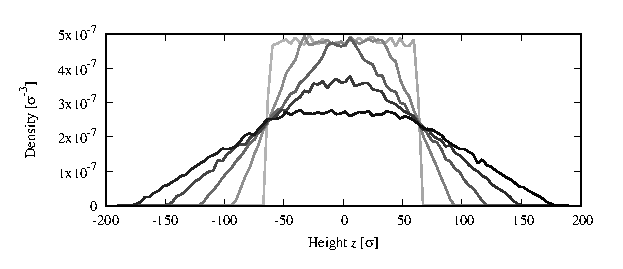
\includegraphics[width = \textwidth]{figures/density.eps}
  \caption{\label{density}Numerical density of particles (number of particles 
           per unit of volume) versus height $z$ for the ideal gas expansion of 
           Figure \ref{freeExpansion}. Darker lines plot later times.}
\end{figure}

\begin{comment}
\begin{lstlisting}
%! codefile: code/density.cu
# include <iostream>
# include "uammd.cuh"
# include "Integrator/VerletNVE.cuh"

using namespace uammd;
using std::make_shared;
using std::endl;

%! codeinsert: density

%! codeinsert: densityPrepareBins

%! codeinsert: densityFillBins

%! codeinsert: densityOutput

int main(int argc, char *argv[]){

  auto sys = make_shared<System>(argc, argv);

  %! codeinsert: particleData src: chapters/first_simulation.tex

  %! codeinsert: initialConditions src: chapters/first_simulation.tex

  %! codeinsert: VerletParams src: chapters/first_simulation.tex

  %! codeinsert: Verlet src: chapters/first_simulation.tex

  std::string outputFile = "density.dat";

  int numberOfSteps = 10000;
  int printEverynSteps = 2000;

  for(int step = 0; step < numberOfSteps; ++step) {
    integrator->forwardTime();

    if(printEverynSteps > 0
       and step % printEverynSteps == 1) {
      auto position
        = particles->getPos(access::location::cpu,
                            access::mode::read);

      density(outputFile, L*L,
              numberOfParticles, position.raw(),
              -real(1.5)*L, real(1.5)*L, 100);
    }
  }

  sys->finish();

  return 0;
} //!
%! codeend !//
\end{lstlisting}
\end{comment}

Concerning the microscopic structure of the system, you could calculate the 
radial distribution function, as in Figure \ref{Lennard-Jones.rdf}, or, if you 
wished to study the dynamics of molecules, their mean square displacement or the 
time correlations of their velocities. Once you have learned how to access the 
microscopic configuration, you can easily write functions that spit out the 
value you wish to measure. Most of these functions contain nothing peculiar to 
UAMMD, so you could write them as external programs that process the data files 
output by UAMMD.

Compare the \texttt{density} function to \texttt{getTotalEnergy}. We could 
include the former in an external program that reads a file containing output 
configurations. The algorithm would not depend on any UAMMD code. By contrast, 
an external program calculating the total energy would need to know all the 
velocities and also possess a copy of the \texttt{Interactor} code for the 
energies. If you decided to modify the \texttt{Interactor} in the UAMMD module, 
then you would have to apply the same change to the external program. I hope you 
realise, therefore, that calculating the energy within your module will 
generally be more convenient, while you can save other measurements like the 
density or radial distribution function for post-processing.

\section{Pressure}

There are several different ways of gauging the pressure of a simulated system. 
For swarms of particles interacting through pair potentials in a periodic 
simulation box, the virial route has probably become the most popular. Let 
$\mathbf{r}_{ij}$ represent the vector from particle $i$ to particle $j$ and 
$\mathbf{F}_{ij}$ the force on $i$ due to its interaction with $j$, then you can 
define the instantaneous pressure as
\begin{equation*}
  P = \frac{N}{V} k_B T
      + \frac{1}{6V} \sum_{i \neq j} \mathbf{r}_{ij} \cdot \mathbf{F}_{ij},
\end{equation*}
with $N$ the number of particles, $V$ the simulation box volume, and $k_B T$ the 
thermal energy. Here we have a good example of a magnitude that we will usually 
want to calculate as the simulation proceeds, because it depends on the 
interactions of every pair of particles.

UAMMD does not include default pressure measurements for its forces, but it does 
provide the infrastructure to build your own. Instead of rewriting Lennard-Jones 
to illustrate how to add the virial calculation in, let us seize this 
opportunity to incorporate a brand new potential function to our library.

The Buckingham potential between particles separated by a distance $r$ equals
\begin{equation*}
  V(r) = Ae^{-Br} - \frac{C}{r^6}.
\end{equation*}
It models the Pauli exclusion principle and Van der Waals interactions slightly 
more realistically than Lennard-Jones potentials, at the cost of a more 
expensive computation.

In the constructor, apart from setting the parameters in the potential, we will 
shift the potential upwards to avoid a discontinuity at the cut-off distance 
\texttt{rc}.
\begin{lstlisting}
%! codeblock: BuckinghamPotential
struct Buckingham {
  real A, B, C;
  real rc;
  real shift;

  Buckingham(real i_A, real i_B, real i_C, real i_rc):
             A(i_A), B(i_B), C(i_C), rc(i_rc) {
    real invr2 = real(1.0)/(rc*rc);
    real invr6 = invr2*invr2*invr2;
    shift = A*expf(-B*rc) - C*invr6;
  }

  real getCutOff() { return rc; } //!
%! codeblockend !//
\end{lstlisting}

The \texttt{ForceEnergy} structure parallels the one we wrote for the Morse 
potential in the previous chapter. The force equals
\begin{equation*}
  \mathbf{F}(\mathbf{r})
    = -\nabla V(r)
    = \left(\frac{BAe^{-Br}}{r} - \frac{6C}{r^8}\right) \mathbf{r}.
\end{equation*}
If we want to calculate the force on particle $i$ due to its interaction with 
particle $j$, then $\mathbf{r}$ above would represent the vector from 
$\mathbf{r}_j$ to $\mathbf{r}_i$, which points in the direction opposite to 
$\mathbf{r}_{ij}$. This explains why we have flipped the signs in the 
expression for the force below.
\begin{lstlisting}
%! codeblock: BuckinghamForceEnergy
  struct ForceEnergy {
    real4 * force;
    real * energy;
    Box box;

    real A, B, C, rc, shift;

    ForceEnergy(Box i_box, real i_rc,
                real4 * i_force, real * i_energy,
                real i_A, real i_B, real i_C, real i_shift):
                box(i_box), rc(i_rc),
                force(i_force), energy(i_energy),
                A(i_A), B(i_B), C(i_C), shift(i_shift) {}

    __device__ real4 compute(real4 ri, real4 rj){
      const real3 rij = box.apply_pbc(make_real3(rj)-make_real3(ri));
      const real r2 = dot(rij, rij);
      if(r2 > 0 and r2 < rc*rc) {
        const real r = sqrtf(r2);
        const real AexpmBr = A*expf(-B*r);
        const real invr2 = real(1.0)/r2;
        const real invr6 = invr2*invr2*invr2;
        return make_real4((-B*AexpmBr/r + 6*C*invr6*invr2)*rij,
                          AexpmBr - C*invr6 + shift);
      }
      return real4();
    }

    __device__ void set(int id, real4 total){
      force[id] += make_real4(total.x, total.y, total.z, 0);
      energy[id] += real(0.5)*total.w;
    }
  }; //!
%! codeblockend !//
\end{lstlisting}

Now we will add a new transverser to the potential, to deal with the calculation 
of the virial. We will need to compute terms of the following form:
\begin{equation*}
  \mathbf{F}_{ij} \cdot \mathbf{r}_{ij}
    = \left(BAe^{-Br}r - \frac{6C}{r^6}\right).
\end{equation*}
\begin{lstlisting}
%! codeblock: BuckinghamVirial
  struct Virial {
    real4 * position;
    real * virial;
    Box box;

    real A, B, C, rc;

    Virial(Box i_box, real i_rc,
           real4 * i_position, real * i_virial,
           real i_A, real i_B, real i_C):
           box(i_box), rc(i_rc),
           position(i_position), virial(i_virial),
           A(i_A), B(i_B), C(i_C){}

    __device__ real compute(real4 ri, real4 rj){
      const real3 rij = box.apply_pbc(make_real3(rj)-make_real3(ri));
      const real r2 = dot(rij, rij);
      if(r2 > 0 and r2 < rc*rc) {
        const real r = sqrtf(r2);
        const real AexpmBr = A*expf(-B*r);
        const real invr2 = real(1.0)/r2;
        const real invr6 = invr2*invr2*invr2;
        return B*AexpmBr*r - 6*C*invr6;
      } else {
        return real(0.0);
      }
    }

    __device__ void set(int id, real total){
      virial[id] += total;
    }
  }; //!
%! codeblockend !//
\end{lstlisting}

The potential ends with two \texttt{getTransverser} functions.
\begin{lstlisting}
%! codeblock: BuckinghamGetTransversers
  ForceEnergy getForceEnergyTransverser(Box box, std::shared_ptr<ParticleData> sys){
    auto force = sys->getForce(access::location::gpu,
                               access::mode::readwrite).raw();
    auto energy = sys->getEnergy(access::location::gpu,
                                 access::mode::readwrite).raw();
    return ForceEnergy(box, rc, force, energy, A, B, C, shift);
  }

  Virial getComputeTransverser(Box box, std::shared_ptr<ParticleData> sys) {
    auto position = sys->getPos(access::location::gpu,
                                access::mode::read).raw();
    auto virial = sys->getVirial(access::location::gpu,
                                 access::mode::readwrite).raw();
    return Virial(box, rc, position, virial, A, B, C);
  }
}; //!
%! codeblockend !//
\end{lstlisting}
As you can see, the virial will be calculated by a generic ``compute'' function. 
The result for each particle ends up in the virial array stored in 
\texttt{particleData}. Let us write a simple function to measure the system 
virial.
\begin{lstlisting}
%! codeblock: getTotalVirial
double getTotalVirial(std::shared_ptr<ParticleData> particles){
  auto virial
    = particles->getVirial(access::location::cpu,
                           access::mode::read);

  double totalVirial = 0.0;

  for(int i = 0; i < particles->getNumParticles(); ++i) {
    totalVirial += virial[i];
  }

  return totalVirial;
}
%! codeblockend !//
\end{lstlisting}

When Ra\'ul P\'erez wrote UAMMD, he did not know in advance how you would like 
to use his generic compute function, so he could not make many assumptions 
regarding when it should run or how it should initialise values. He left that up 
to you.

In this case, we have to run our function before we calculate the virial. We'll 
add it into our sampling loop. We'll begin by clearing the virial vector, then 
we'll calculate the temperature and pressure, and we'll end by print out the 
results.
\begin{lstlisting}
%! codeblock: BuckinghamSampling
if(printEverynSteps > 0
       and step % printEverynSteps == 1) {
      {
        auto virial
          = particles->getVirial(access::location::cpu,
                                 access::mode::write);

        std::fill(virial.begin(), virial.end(), real(0.0));
      }

      interaction->compute(0);

      real thermalEnergy = getThermalEnergy(particles);
      real totalVirial = getTotalVirial(particles);
      real volume = box.boxSize.x*box.boxSize.y*box.boxSize.z;
      real pressure = particles->getNumParticles()*thermalEnergy/volume
                      + totalVirial/(6*volume);

      auto position
        = particles->getPos(access::location::cpu,
                            access::mode::read);
      const int * index = particles->getIdOrderedIndices(access::location::cpu);

      out<<endl;
      for(int id = 0; id < numberOfParticles; ++id)
        out<<box.apply_pbc(make_real3(position[index[id]]))<<endl;

      macro<<step*VerletParams.dt<<" ";
      macro<<getTotalEnergy(integrator, particles)<<" ";
      macro<<getTotalMomentum(particles)<<" ";
      macro<<thermalEnergy<<" "<<pressure<<endl;
    } //!
%! codeblockend !//
\end{lstlisting}
We usually define interactors within a block of code set apart by brackets. If 
we did the same here, then the program  would not work because we need the 
variable \texttt{interactor} to be defined in the sampling loop. Therefore, we 
need an active instance of the Buckingham interactor in our main function. For 
example, if we wished to measure the state of \textsuperscript{4}He atoms, we 
could write something like this:
\begin{lstlisting}
%! codeblock: BuckinghamInteractor
  real A = 37101;
  real B = 4.4148;
  real C = 113.09;
  real rc = 6.0;

  auto BuckinghamPotential = make_shared<Buckingham>(A, B, C, rc);

  using BuckinghamForces = PairForces<Buckingham>;
  BuckinghamForces::Parameters interactionParams;
  interactionParams.box = box;

  auto interaction
    = make_shared<BuckinghamForces>(particles, sys,
                                      interactionParams,
                                      BuckinghamPotential);

  integrator->addInteractor(interaction); //!
%! codeblockend !//
\end{lstlisting}
I found the values for the Buckingham potential parameters in the work of 
Ko\v{c}i \textit{et al.}, \textit{Study of the high-pressure helium phase 
diagram using molecular dynamics} (J. Phys.: Condens. Matter \textbf{19}, 
016206, 2007). As a simple check, I ran the code and found that the 
\textsuperscript{4}He equilibrated at a temperature of about $130\ \mathrm{K}$, 
a pressure of $0.18\ \mathrm{GPa}$ and a volume of $16\ 
\mathrm{cm}^3/\mathrm{mol}$, compatible with the work of these authors.

\begin{comment}
%! codefile: code/Buckingham.cu
%! codeinsert: includeGenericMD
%! codeinsert: includeLennard-Jones
# include "Integrator/VerletNVE.cuh"

%! codeinsert: namespaceUAMMD

%! codeinsert: BuckinghamPotential

%! codeinsert: BuckinghamForceEnergy

%! codeinsert: BuckinghamVirial

%! codeinsert: BuckinghamGetTransversers

%! codeinsert: getTotalEnergy

%! codeinsert: getTotalMomentum

%! codeinsert: getThermalEnergy

%! codeinsert: getTotalVirial

int main(int argc, char * argv[])
{

  auto sys = make_shared<System>(argc, argv);

  int numberOfParticles = 10000;
  auto particles
    = make_shared<ParticleData>(numberOfParticles, sys);

  real L = 64;

  Box box(make_real3(L, L, L));
  bool periodicityX = true, periodicityY = true,
       periodicityZ = true;
  box.setPeriodicity(periodicityX, periodicityY,
                     periodicityZ);
  {
    auto position
      = particles->getPos(access::location::cpu,
                          access::mode::write);

    auto initial =  initLattice(box.boxSize,
                                numberOfParticles, sc);

    std::copy(initial.begin(), initial.end(), position.begin());
  }

  {
    auto mass
      = particles->getMass(access::location::cpu,
                           access::mode::write);

    std::fill(mass.begin(), mass.end(), real(1.0));
  }

  using Verlet = VerletNVE;
  Verlet::Parameters VerletParams;
  VerletParams.dt = 0.001;
  VerletParams.initVelocities = true;
  VerletParams.energy = 2.0;

  auto integrator
    = make_shared<Verlet>(particles, sys, VerletParams);

  %! codeinsert: BuckinghamInteractor

  std::string outputFile = "helium.dat";
  std::ofstream out(outputFile);

  std::string macroFile = "heliumMacro.dat";
  std::ofstream macro(macroFile);

  int numberOfSteps = 10000;
  int printEverynSteps = 100;

  for(int step = 0; step < numberOfSteps; ++step) {
    integrator->forwardTime();

    %! codeinsert: BuckinghamSampling
  }

  sys->finish();

  return 0;
} //!
%! codeend !//
\end{comment}

\bigbreak

If you braved the chapters leading up to this point, you already know enough to 
set up and run many interesting computations of your own. Now, deciding whether 
your model correctly represents an empirical observation involves a solid 
understanding of the relevant physics. Some simulations may seem to work fine 
but then display a completely different behaviour from the actual experiment. As 
an example of the type of subtle theoretical difficulties that may arise, I have 
dedicated the next chapter to long-range interactions.

\begin{comment}
List of programs written in this chapter:
%! codeblock: codelist
* `rubberBallE.cpp`: A version of the `rubberBall.cpp` from the introduction
   which also outputs the mechanical energy of the ball (*section*: 3.1).
* `measurements.cu`: An improvement of `superLennard-Jones.cu` that outputs the
   total energy and linear momentum, and the thermal energy, which is
   proportional to the absolute kinetic temperature (*sections*:
   3.1&ndash;3.2).
* `checkpoints.cu`: An extension of `measurements.cu` with the ability restore
   simulations from saved checkpoints (*section*: 3.3).
* `Langevin.cu`: Lennard-Jones molecular dynamics simulation with a Langevin
   thermostat (*section*: 3.4).
* `Brownian_dynamics.cu:`: Brownian dynamics simulation with Lennard-Jones
   interactions (*section*: 3.5).
* `shear.cu:`: Brownian dynamics simulation with Lennard-Jones particles
   suspended in a shear flow (*section*: 3.5).
* `Andersen.cu`: Lennard-Jones molecular dynamics simulation with an Andersen
   thermostat (*section*: 3.6).
* `Euler.cu`: Lennard-Jones molecular dynamics integrated with the Euler scheme
   (*section*: 3.6).
* `density.cu`: Density profile of the ideal free gas expansion from sections
   1.1&ndash;1.4 (*section*: 3.7).
* `Buckingham.cu`: Helium atoms interacting through the Buckingham potential in 
   a simulation that measures the pressure (*section*: 3.8).
%! codeblockend
\end{comment}

